%%%% ijcai19-multiauthor.tex

\typeout{IJCAI-19 Multiple authors example}

% These are the instructions for authors for IJCAI-19.

\documentclass{article}
\pdfpagewidth=8.5in
\pdfpageheight=11in
% The file ijcai19.sty is NOT the same than previous years'
\usepackage{ijcai19}

% Use the postscript times font!
\usepackage{times}
\usepackage{soul}
\usepackage{url}
\usepackage[hidelinks]{hyperref}
\usepackage[utf8]{inputenc}
\usepackage[small]{caption}
\usepackage{graphicx}
\usepackage{amsmath}
\usepackage{booktabs}
\urlstyle{same}

\usepackage[utf8]{inputenc}
\usepackage[english]{babel}
\usepackage{multicol}
\usepackage{enumitem}
\usepackage{graphicx}
\usepackage{pgfplots,booktabs}
\usepackage{booktabs,caption}
\usepackage{threeparttable}
\usepackage{amsmath}
\usepackage{amssymb}
\usepackage{longtable}
\usepackage{afterpage}
\usepackage{float}
\usepackage{titlesec}


\title{Optimizing online documents for fact-checking\\
A Machine Learning Application\\
Research Paper\\}

\author{
Alexander Peikert\footnote{218200812}\and
Clemens Steinmann\footnote{218200209}\and
Erwin Letkemann\footnote{218200352}\And
Julian Dillmann\footnote{218100919}\\
\affiliations
\textbf{WeST} \\
\textbf{Universität Koblenz-Landau} \\
\textbf{Group:} Alpha

\emails
alexpeikert@uni-koblenz.de,
csteinmann@uni-koblenz.de,
erwinletkemann@uni-koblenz.de,
juliandillmann@uni-koblenz.de
}
\begin{document}

\maketitle

\begin{abstract}
In this application we present a tool to find verified claims for a given input claim.
The problem at hand is defined as in Clef2020! Task 2\cite{DBLP:conf/ecir/Barron-CedenoEN20} Verified claim retrieval.
To solve the task we build a model based on Elasticsearch\footnote{https://www.elastic.co/} to retrieve verified claims and a tuned Sentence-Bert\cite{DBLP:conf/emnlp/ReimersG19} model to re-rank the retrieved claims.\\
This approach was transformed into verified claims database, in order to retrieve and rank claims given an import source such as a news article.
The application is intended to be used as tool to help the process of verifying claims on the web, by speeding up the process of identifying whether a claim was verified before or not.

\end{abstract}

\section{Introduction}
\subsection{Problem}
%--------------------------
% Introduction
%--------------------------
Indefinitely amount of data is created each day combined with the easy access and possibilities to publish and spread information for everybody, it is getting difficult to easily distinguish between genuine information sources and those that try to misinform.
Although there are organizations that conduct fact-checking, the time it takes to verify statements is far greater than the time it takes for a new content that needs to be verified to originate.\\
In that case a fully automated system to detect and fact check claims on the web sounds like a good idea, but in practice the work needed for a single fact-check is to complex for a computer system.
The vastly different contexts and the needed sensitivity that is needed to judge claims, can only be comprehended by humans.
Ideally the process of manual fact-checking should be improved, to speed up sub tasks that are performed in fact-checks, by developing and providing tools for fact-checkers. Such as checking claims against authoritative sources or checking claims against previously fact-checked claims \cite{graves2018a}.
%--------------------------
% Motivation
%--------------------------
\subsection{Goal}
Our goal is to provide a web-based service to speed up the process of manual fact-checking for fact checkers in different organizations. 
The tool should provide an additional way for fact checkers to automatically find if claims have been already fact checked before, by other organizations, besides their internal collection of data.
Apart from that the application should also represent a service for ordinary web users that are interested in fact-checking to have an easy to use service to find verified claims for internet news content. 
%--------------------------
% Application example
%--------------------------
\subsection{Application}
The application will work as follows:
The user inputs a URL or text of a news source on the applications website.
The service retrieves relevant verified claims from the database of already verified claims.
The retrieved claims are scored based on relevance to the sentences.
The website will display the top ranked retrieved claims for each sentence that provide help in verifying the news article.
The website can also be used to retrieve the most matching claims for example form a single sentence.
More detailed explanation in methodology.



%--------------------------
% Related Parents
%--------------------------
\section{Related work}
On the subject of "claim retrieval" is currently worked on for example in CLEF CheckThat 2020\cite{DBLP:conf/ecir/Barron-CedenoEN20}.
Most earlier work in the area of automatic fact checking was done on the topic of identification of "check worthy" statements or articles.
ClaimPortal\footnote {https://idir.uta.edu/claimportal/}\cite{DBLP:conf/acl/MajithiaALJACL19} is such an instance where tweets from several US politicians are analyzed and assigned with a check worthiness score, in the regard if the factual claim in the post, if present, is of importance for the public.\\
There is also ClaimReview\footnote{https://www.claimreviewproject.com/} a tagging system to identify fact-checked articles.
This framework to structure data provides help for machines to interpret fact-checks on articles.\\
Research on determining the check worthiness of political claims was also done with the help of nutritional labels and word embedding\cite{DBLP:conf/sigir/LespagnolMU19}.
The authors used models in natural language processing to determine the nutritional labels and also used Word2Vec model to determine key words in sentences.
They hypothesized a correlation between the different implications of the labels and the veracity of claims, for example high emotions in political statements indicate an attempt to deceive the audience.
Hence the statement should be check worthy. 
All three of these were used in different combinations in several different ML algorithms to evaluate the performance on the CheckThat! 2018 \cite{DBLP:conf/clef/NakovBESMZAKM18} dataset.
The authors concluded that the nutritional labels with word-embedding with stochastic gradient descend logless without oversampling  archived the best MAP\footnote{Mean Average Precision} of all the combinations of possible inputs with different algorithms.
At the same time their solution outperformed or matched the best participants' methods on MAP, MRR\footnote{Mean Reciprocal Rank} and MP@5.\\
These results showcase that nutritional labeling could be of use in further research in computational detection of misinformation in a bigger range of topics or automated help tools for manual fact checking.\\
On the topic of natural language processing Transformer models such as Bert\cite{DBLP:conf/naacl/DevlinCLT19} improved performance of NLP tasks. In Transformer models for each term the terms before and after are considered in creating the embedding thus improving understanding of language context.
This network provides a basis to purpose train a model for specific nlp task, achieving state of the art performance in the respective task.\\
Sentence-Bert\cite{DBLP:conf/emnlp/ReimersG19} for instance is a modification of Bert to reduce the computation cost for embedding for semantically meaningful embedding at the same accuracy.\\
To solve our problem we take the same approach to use pre-trained model, Sentence-Bert, as a basis for purpose tuning the model for the retrieval and ranking task at hand.
%--------------------------
%Application
%--------------------------
%Database
%--------------------------
\section{Methodology}
\begin{figure}[h]
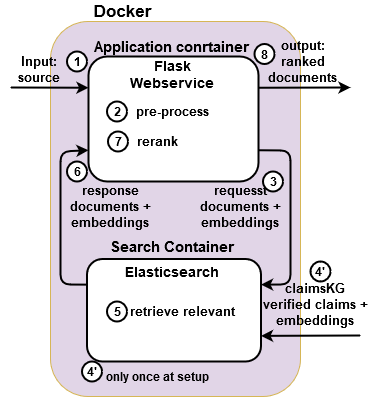
\includegraphics[scale=0.7]{App.png}
\caption{Application structure \& usage flow}
\end{figure}
\noindent\textbf{databases:} 
The search container is based on Elasticsearch mirror of ClaimsKG's\footnote{https://data.gesis.org/claimskg/ } database to support the claim matching algorithm.
Elasticsearch provides an efficient way to text search.
For the search we store the verified claims and additional fields like keywords, named entities etc. that could be helpful identifying documents in the database.
Additionally we  store the verified claim as dense vector in the database to avoid embedding each verified claim several times.
Furthermore content of Politifact\footnote{https://www.politifact.com/} and Snopes\footnote{https://www.snopes.com/} should be able to be scraped and added to the mirror regularly seeing that these represent about 85\% of the current sources for claims in ClaimsKG. \\
%--------------------------
%Preprocessing
%------------------------------------------------------------------------------
\noindent\textbf{labels:}
We also provide nutrition labels style scores if the input is a news article.
These labels such as emotion, controversy, option should provide user help to assessment the contents of the article before reading.
\begin{itemize}
	\item The emotions are determined by a hourglass model \cite{DBLP:conf/cost/CambriaLH11}. By the sum of positive and negative annotated words in the text we assign a label measuring the overall emotions over the text.
	\item Controversy compares the length of the document to the number of topics from list of controversial issues\footnote{Wikipedia:List of controversial issues}.
	\item We analyses sentiment of sentences and the overall number of sentences containing opinions of the text with the help of Vader\cite{DBLP:conf/icwsm/HuttoG14} library.
\end{itemize}
%------------------------------------------------------------------------------------
%Claim matcher
%--------------------------
\noindent\textbf{Web service:}
Our indented use of the application is by providing a website based on flask, or as python package.
The website serves as easy to navigate interface between user and database.
The input is either an already extracted text body of an article or the HTML to the article.
In the second instance the text body is extract with the help of trafilatura\cite{DBLP:conf/konvens/Barbaresi19}, \cite{DBLP:conf/aclwac/Barbaresi16} library.
By default the user should paste the text body because the scraping can be broken on some domains.
As output the application would provide the top ranked matching claims form ClaimsKG either for each sentence, or over for the whole text.
We also provide the possibility to summarize the text, in order to decrease the run time for the application, due to the increased computation time that scales with the number of sentences to check. \\
\noindent\textbf{claim scoring:}
The core of the application is the claim matching.
In this process we find and rank claims from the ClaimsKG database that support the claim in question.
ClaimsKG is a structured database that collects claims and metadata from popular fact-checking organizations/ sites. 
Currently they provide access to 33623 verified claims from 9 different sources, notably Politifact and Snopes,  with four different classification levels. 
True and false, and two measures, to compress the different classification metrics of different fact-check providers, that don't satisfy either true or false completely.\\
To inspect the details, the claim matching is set up in three parts.
First a model based on term frequency of the query in the extracted claims is used to determine Boolean relevancy of the verified claims.
This step is required to greatly decrease the number of documents for further computation in the second step.
ClaimsKG already provides 12297 unique keywords to help with the matching.
Additionally a score based on term-frequency inverse document frequency is computed by Elasticsearch in the search process to pre-rank the documents based on query terms.
The next step the claims are compared, by the semantic similarity of the query claim and the retrieved claims with the help of the Transformer model.
For the final rank we normalize both scores, elastic search term based and cosine similarity score, compute a weighted sum of them.
The documents are re-ranked after this new score.\\
%----------------------------
% Training
%----------------------------
\noindent\textbf{Training:}
We used the Distilbert\cite{DBLP:journals/corr/abs-1910-01108}-nli-stsb-mean model as base.  
This model is an already pre-trained Transformer based sentence embedding method, that was already tuned on natural language interference and semantic text similarity.\\
We used the clef Check!That 2020\cite{DBLP:conf/ecir/Barron-CedenoEN20} Task 2 data set containing 10325 claims and 997 tweets with matching tweet claim pairs to tune the model.
In addition to the one matching claim, we randomly sampled 99 further claims as negative samples from the verified claims.
We used contrastive loss function and Binary classification evaluation for / during training, and cosine similarity as distance measure between the pairs. 
That means for the positive pair of (tweet, positive claim) the weights of the transformer are decreased and for the negative pairs (tweet, negative claim) the weights are increased during training.
For the training we used 800 samples from the training set and periodically evaluated the models performance on the remaining unknown pairs with Binary classification to classify the claims as positive or negative match.\\
We also tuned a separate model on triplet loss function and triplet evaluation.
There we provide (tweet, positive, claim, negative claim) pairs and the weights are increased and decreased similar as above.\\
The script for training was used from sentence-bert\footnote{https://github.com/UKPLab/sentence-transformers}.\\
\noindent\textbf{Evaluation:}
For evaluation we use the same data set provided by the CheckThat! 2020 Task 2. 
Our evaluation main metrics are mean average precision at 5 and 1.
The aim is to retrieve relevant verified claims for tweets/shot sentence\footnote{for the remainder of the Evaluation we refer to these as tweets}. 
The evaluation data set provides 197 tweets to 10375 verified claims.
For each tweet there is one matching verified claim, all other claims are assumed not relevant for a given tweet.\\
The script for evaluation was used from Clef Task\footnote{https://github.com/sshaar/clef2020-factchecking-task2}.
%----------------------------
%Evaluation
%----------------------------
\section{Evaluation}
\subsection{Baseline}
The baseline, we compare to, uses Elasticsearchs build in search tool as scoring function. Elasticsearch is build on Lucene\footnote{https://lucene.apache.org/}.
As short introduction to relevance scoring in Elasticsearch, a higher score means higher relevance of a document given a query. Before scoring any document all relevant documents are retrieved by a Boolean query.
The remaining documents are scored based on a combination of term-frequency (tf), inverse document frequency (idf), field-length normalization to calculate the terms weight in a document, and for multi-term queries a vector space model based on the tf-idf to compare query and documents.
Furthermore there the other factors that can be applied to influence relevance, for example by providing a boosting factors like queries, terms or fields.
To wrap-up, our baseline uses a vector space model based on tf-idf, and no additional boosting etc., to rank the retrieved documents for the similarity scoring between a given tweet and the verified claims. The scores are dynamically assigned during the query indexing in Elasticsearch.
That means our baseline only considers textual similarity of the tweet terms and does not consider semantic similarity or any other measure to rank verified claims.
\subsection{Model results}
Our model introduces semantic similarity into the ranking of the retrieved documents.
We rank the documents based on a weighted sum of cosine similarity of embedding created by the fine-tuned Transformer model based on Distilbert-nli-sts and the tf-idf term score as in the baseline.
\begin{table}[H]
\centering
\begin{threeparttable}
    \begin{tabular}{lrrr}
        \toprule
         & Baseline & Our  \\ \midrule
        MAP@1 		& 0.470 & 0.713  \\
	  MAP@3 		& 0.601 & 0.789 \\
        \textbf{MAP@5} & 0.609 & \textbf{0.789} \\
        MAP 			& 0.619 & 0.798 \\ \bottomrule
   \end{tabular}
\caption{Comparing our model to baseline.\\}
\end{threeparttable}
\end{table}
\noindent Noteworthy even if our main measure for evaluation is Mean Average Precision at 5 in our model retrieves with the same Precision at 3.
\subsection{Experiments}
\subsubsection{Building of our Model }
To begin we used sentence transformers to calculate the embedding for the vector space model in order to compare tweet and verified claim.
The comparison of the embedded sentences is done by cosine similarity.\\
We need to decide which model to use, therefore we compared pre-trained Transformer models to the baseline.
Both models that we considered where  trained on Natural Language Interference\cite{DBLP:conf/emnlp/BowmanAPM15} data set (NLI) and fine-tuned Semantic Textual Similarity\cite{DBLP:conf/semeval/CerDALS17} (STSb) data set.\\
The following evaluations are always going to be of the top 500 scored documents.
That means the 500 documents are rank is based on the elastic score described as above. For the Transformer models we use the same Elasticsearch architecture to retrieve relevant documents and afterwards re-rank these 500 documents by computing the cosine similarity between tweet and embedding.\\ 
\begin{table}[H]
\centering
\begin{threeparttable}
    \begin{tabular}{lrrr}
        \toprule
         & Baseline & Bert & Distilbert \\ \midrule
        MAP@1 		& 0.470 & 0.388 & 0.368 \\
	  MAP@3 		& 0.601 & 0.503 & 0.475\\
        \textbf{MAP@5} & \textbf{0.609} & 0.511 & 0.492\\
        MAP 			& 0.619 & 0.529 & 0.504 \\ \bottomrule
   \end{tabular}
\caption{Comparing pre-trained model to baseline.\\}
\end{threeparttable}
\end{table}
\noindent Considering that the models were already pre-trained with STS, and performing well in the corresponding STS benchmark\footnote{Spearman score of ~ 85+ in STSb.}, they do not perform well in this retrieval task.
We further fine-tune the model with the training data to improve performance in the specified task.\\
We need to purpose tune the base models to fit our task.
The fine-tune is done as described in Methodology.
After fine-tuning the models and using the method to re-rank the 500 retrieved documents, we get the following results:
\begin{table}[H]
\centering
\begin{threeparttable}
    \begin{tabular}{lrrr}
        \toprule
         & Distilbert\tnote{1} & Distilbert\tnote{2} & Bert\tnote{3} \\ \midrule
        MAP@1 		& 0.642 & 0.604 & 0.431 \\
	 MAP@3			& 0.703 & 0.671 & 0.523 \\
        \textbf{MAP@5} & \textbf{0.715} & 0.688 & 0.538 \\
        MAP 			& 0.727 	& 0.699 & 0.557 \\ \bottomrule
   \end{tabular}
\begin{tablenotes}\footnotesize
\item Note: Bert was fine-tuned with a batch size of 16 instead of 32. 
\item[1] Contrasive loss
\item[2] Triplet loss
\item[3] Contrasive loss
\end{tablenotes}
\caption{Comparing different loss functions.}
\end{threeparttable}
\end{table}
\begin{table*}[t]
\centering
    \begin{tabular}{lrrrrrrr}
        \toprule
        p 				& 0.3     & 0.5    & 0.6     & 0.7     & 0.75   & 0.8    & 0.85 \\ \midrule
        MAP@1 		& 0.622 & 0.668 & 0.693 & 0.703 & 0.713 & 0.713 &	 0.708	\\
	 MAP@3		 	& 0.714 & 0.756 & 0.781 & 0.786 & 0.789 & 0.784 & 0.781 \\
        \textbf{MAP@5} & 0.718 & 0.759 & 0.782 & \textbf{0.787} & \textbf{0.789} &  \textbf{0.788} & 0.782	\\
        MAP 			& 0.727 & 0.768 & 0.790 & 0.796 & 0.798 & 0.796 & 0.791	\\ \bottomrule
   \end{tabular}
\caption{Comparing different values for parameter p.}
\end{table*}
\noindent We can observe that the Distilbert model is performing better after fine-tuning with the same loss function.
Comparing the performance of the different loss functions in training, we can see that contrastive loss slightly outperforms Triplet loss.
Furthermore looking back at the baseline and base models, for Distilbert tuning notable improves the model. In case of the Bert training the fine-tuned model did not significantly improve the untrained model and also still falls behind the baseline.
We concluded that this behavior is due to the lower batch size that we used in training due to higher memory demand.\\
We decided to continue with the Distilbert model due to a lower resource and time consumption for tuning and embedding.\\
Just relying on cosine similarity we have the problem, that tweets and document pairs, do not necessary share exact semantics and a high likelihood of another non relevant documents having a higher cosine score.
Also having tf-idf weight for uncommon words is beneficial in information retrieval systems.
Therefore we combine both the score provided by the Elasticsearch and the cosine similarity into one score for ranking.\\
The new score is the min-max normalized sum of both scores.
Additionally we introduce a parameter $0\leqslant p \leqslant1$ to express the importance of one of the scores over the other.\\
The new score is :
\begin{equation*}
\begin{aligned}
Score & = p \cdot \frac{cosine(query_{embedding}, vclaim_i) - min_{vclaim}}{max_{vclaim} - min_{vclaim}} + \\
& (1-p) \cdot \frac{elastic_i - min_{elastic}}{max_{elastic} - min_{elastic}}\\
\end{aligned}
\end{equation*}
$query_{embedding}$\quad vector representation of of query.\\
$vclaim_i$ \quad vector representation of i-th retrieved document Fgiven query.\\
$elastic_i$ \quad Elasticsearch score of i-th retrieved document given query.\\
$max,\,min$ \quad respective max and min values of scores for a query.\\ 
$0\leqslant p \leqslant1$ \\
For a value of 0.5 for p Elasticsearchs tf-idf score and the cosine similarity score created by the Transformer model are considered equally for the final result score.
For values bigger than 0.5 the cosine similarity is considered more in the end result, and for values less than 0.5 the other way around.\\
Looking at the Elasticsearch tf-idf ranking score we can observe that for most high matched documents the scores are within margin of each other, with the exception of occasionally a outlier that is several times higher.
Such an outlier would corresponds to a rare term in the retrieved document/claim which likely means that it is indeed the relevant claim. 
Cosine similarity would not specifically score that document higher compared to other documents.
With the new score we can combine both the general performance improvement of cosine similarity and the better detection of rare terms in documents.\\
In Table 4 we see that as expected the performance increases if we consider cosine similarity more in the final result.
This was expected due the higher base performance of the fine-tuned models over the baseline. 
For the parameter p the range $0.7\leqslant p \leqslant0.8$ yields the best performance in the task.
\subsubsection{Other} 
During training we experimented with different sizes of the number of negative samples for the training samples besides the one positive document to tune the model.
The following models were fine-tunes of the Distilbert model as above with the contrastive loss function and evaluated based on cosine similarity scoring.
The numbers represent the number of negative pairs + positive pair per tweet in the different training sets (Table 5).
\begin{table}[H]
\centering
\begin{threeparttable}
    \begin{tabular}{lrrrr}
        \toprule
         				& 24+1 & 49+1 & 99+1 & 249+1 \\ \midrule
        MAP@1 		& 0.581 & 0.627 & 0.642 & 0.602 \\
	 MAP@3			& 0.663 & 0.682 & 0.703 &0.687 \\
        \textbf{MAP@5} & 0.678 &0.694 &\textbf{ 0.715} & 0.697 \\
        MAP 			& 0.689 	& 0.709 & 0.727 & 0.709  \\ \bottomrule
   \end{tabular}
\caption{Comparing different number of negative training pairs per tweet.}
\end{threeparttable}
\end{table}
\noindent Furthermore we evaluated the tuned models at with different batch sizes, warm up steps, number of evaluations during training, number of epochs and margins for the distance metric.
We found that all test models performed best at roughly after 2 epochs.
Increasing batch size also improved performance of the models.
\subsection{Application}
Evaluating how well the model in the task performs as real world application on the claimsKG data is difficult to measure.
For one there was no fine-tuning with claimsKG claims, because it is difficult to get proper training samples for positive matches without manually reviewing all articles that were fact-checked on the various fact-check sites that claimsKG gathered. 
Furthermore the number of verified claims 33000+ verified claims are to little to possible cover all claims that can be found in the web.
You could find introduce additional sources for verified claims and knowledge to the database.\\
Some claims are specific to one event for example: Person X said Y about Z at W. 
Such claims are only useful articles on that specific topic however there should not be that many articles about that event after some the event took place.
Also considering new/ current events, e.g political debates, there would likely be no available fact-check depending on how recent the event was.\\
Other improvements that could be made in the pre-processing of articles.
If for example using HTML text extraction can be improved to only retrieve sentences or part of sentences with claims to build the query. 
Besides providing directly providing the desired text sections, this would help decreasing the time per article given the Transformer models computation time scales with the number of sentences to embed.
%----------------------------
\bibliographystyle{abbrv}
\bibliography{paper}



\end{document}











































